% Chapter 1

\chapter{Chapter Title Here} % Main chapter title

\label{Chapter1} % For referencing the chapter elsewhere, use \ref{Chapter1} 

%----------------------------------------------------------------------------------------


%----------------------------------------------------------------------------------------



\section{Our Approach}\label{sec:approach}



\begin{figure}
	\centering
	\begin{minipage}{.5\textwidth}
		\centering
		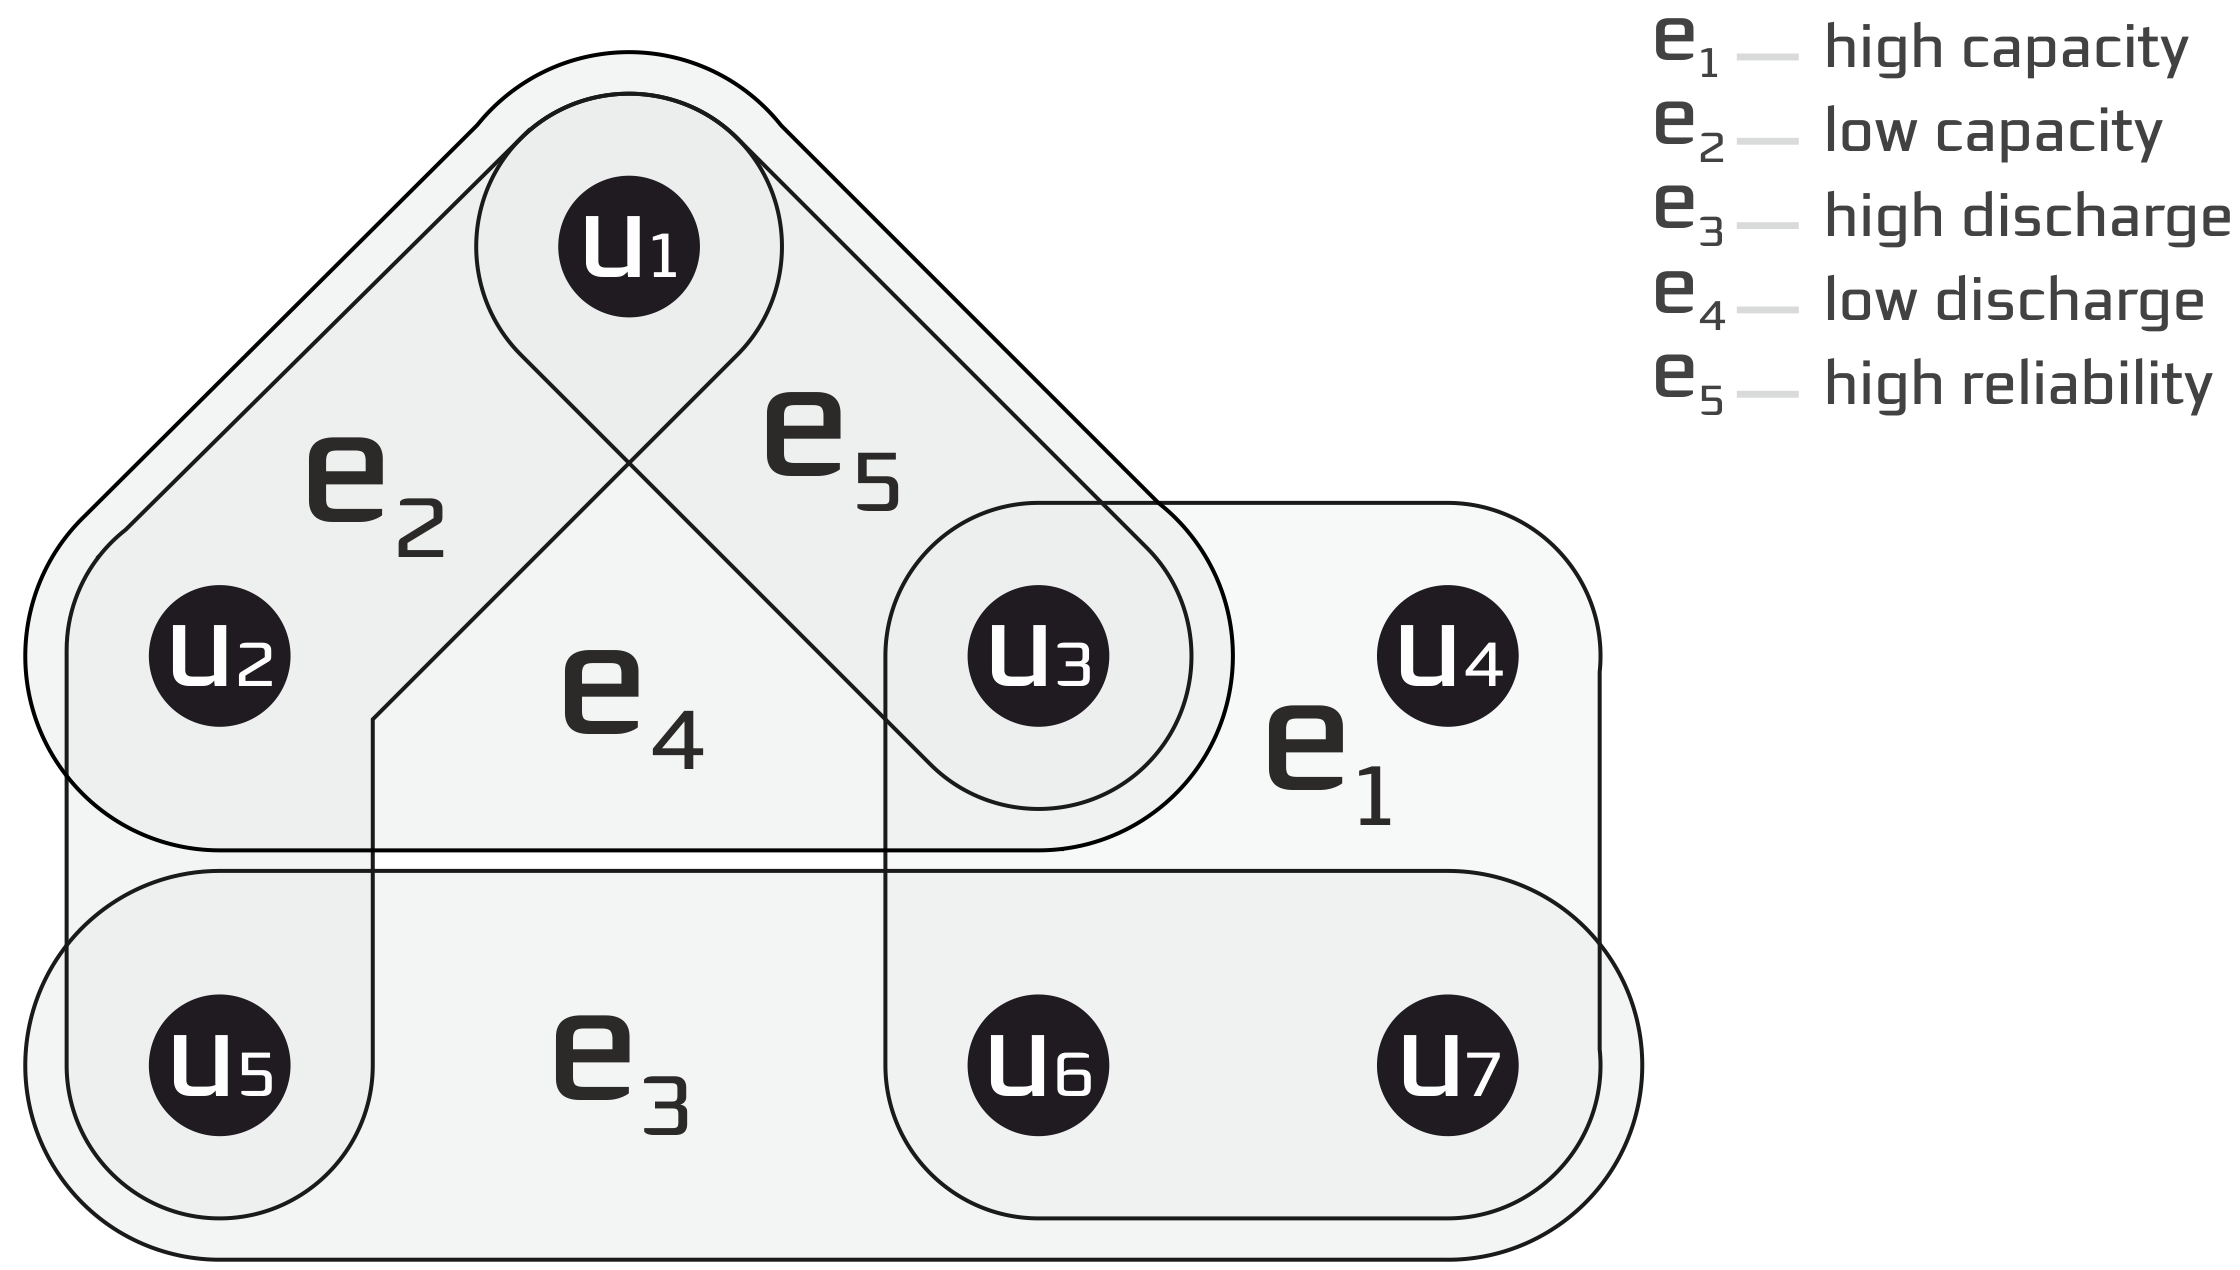
\includegraphics[scale=0.3]{hypergraph.png}
		\caption{A simple hypergraph\label{fig:hypergraph}}
	\end{minipage}%
	\begin{minipage}{.5\textwidth}
		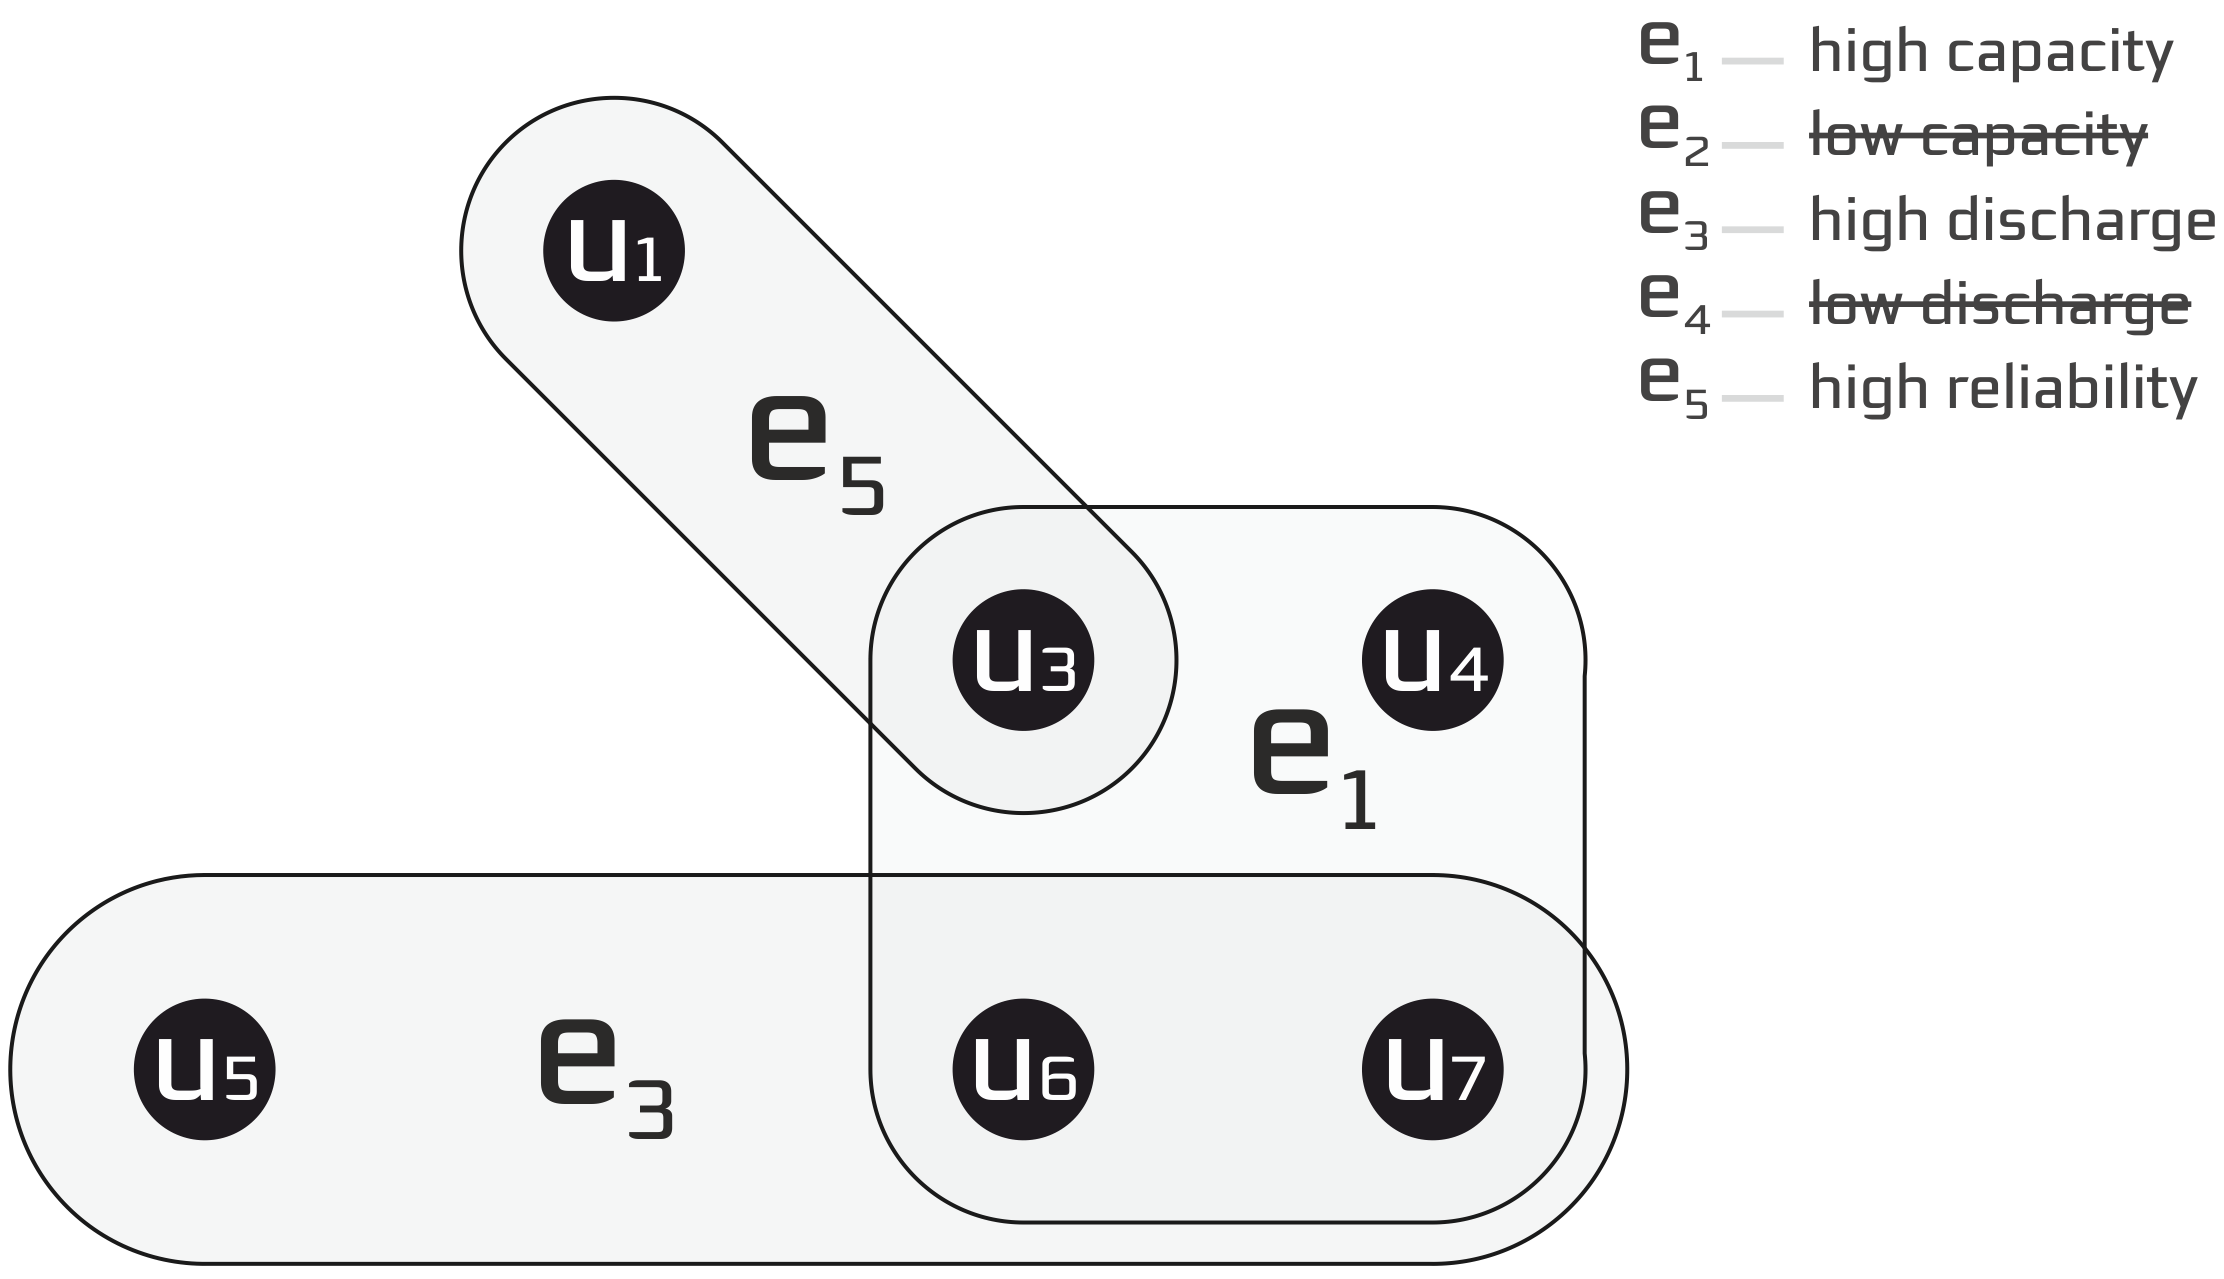
\includegraphics[scale=0.3]{hypergraph_prune.png}
		\caption{Pruning a simple hypergraph\label{fig:hypergraph_prune}}
	\end{minipage}
\end{figure}

In order to develop multi-criteria coalition formation algorithms that generate coalitions efficiently, we employ the concept of {\em a hypergraph}.
A hypergraph $H = (V, E)$ is a generalization of a graph, where each {\em hyperedge} $e \in E$ can contain any number of {\em vertices (or nodes)} in the set $V$.
Vertices in $H$ correspond to agents; while we view a hyperedge as corresponding to some particular {\em attribute} or {\em characteristic} possessed by the agents in the hyperedge.
In the V2G setting, the agents correspond to EVs (i.e., an EV is represented by a node in our hypergraph); while the hyperedges correspond to vehicle characteristics. More specifically, a hyperedge corresponds to a ``quality level'' of some EV attribute, as we explain below.

In order to represent the different {\em quality} of the various hyperedges, and utilize it in our algorithms, we mark each hyperedge with a weight.\footnote{In our implementation, the weight of the edges, according to the quality of each attribute(capacity, reliability and discharge), are as follows: \{\textit{extremely-high: 8, very-high: 7, high: 6, medium-high: 5, medium-low: 4, low: 3,very-low: 2, extremely-low:1}\}. Thus we have 24 edges + 1 containing commitment of EVs.} These weights define the \textit{degree} of a node: {\em The degree $deg(u)$ 
	of a node 
	$u$ 
	is the sum of the weights of its edges}. Intuitively, {\em a high degree node is a high quality one}. This fact is exploited in our algorithms below.
A hyperedge (of a given quality) will be also called a {\em category}. The (quality of the) categories to which an EV belongs will be influencing the decisions of our {\em hypergraph pruning} algorithm, which we describe in Section~\ref{sec:pruning} below. A node that belongs to a hyperedge characterizing the quality of a given agent attribute, cannot belong to some other hyperedge characterizing the quality of the same attribute.


To illustrate the use of hypergraphs in our setting, consider for example the hypergraph of Fig.~\ref{fig:hypergraph}, which contains the hyperedges $e_{1...6}$ and vertices $u_{1...7}$. It is clear in this example that vertices may belong to multiple hyperedges: the hyperedge $e_1$ contains the vertices $u_{3,4,6,7}$, while the vertex $u_1$ belongs in the hyperedges $e_2, e_5, e_4$. Vertices in Fig.~\ref{fig:hypergraph} correspond to EVs; while the hyperedges correspond to the ``quality'' of the following EV attributes: \textit{capacity}, {\em discharge rate} and \textit{observed reliability}. The meaning of these attributes is intuitively straightforward, but will be nevertheless explained in Section~\ref{subsec:criteria} below. Each attribute is related to at least one hyperedge in the hypergraph. For instance, in Fig.~\ref{fig:hypergraph}, the {\em capacity} attribute is represented by three hyperedges in the hypergraph: {\em low-capacity}, {\em medium-capacity}, and {\em high-capacity}. As noted above, no node can belong in more than one capacity-related hyperedges. In our figure, 
\begin{itemize}
	\item the hyperedge $e1$ represents the nodes which have high capacity;
	\item the hyperedge $e2$ contains nodes that have low capacity;
	\item $e3$ and $e4$ include the vehicles with high and low discharge rate, respectively;
	\item finally, $e5$ contains nodes that are expected to the {\em highly reliable}.
\end{itemize}
For example, node $u1$ is a {\em low-capacity}, {\em low-discharge} but {\em highly reliable} vehicle---while node $u3$ is a {\em high-capacity}, {\em low-discharge} and {\em highly reliable} one.

%       A simplified example of how we store attributes of a hypergraph is presented in Figure~\ref{fig:hypergraph}.

%       If we were to simplify our hypergraph to the size of the example, then Figure~\ref{fig:hypergraph} would be our hypergraph with seven nodes $u \in V$ and five hyperedges
% $e \in E$. These nodes would represent vehicles and each hyperedge represents a specific attribute as we can see in the legend.

%       It should be noted that in the hypergraph we used in our experiments, there were several more hyperedges.

Organizing the information relating to specific agent attributes using hyperedges, enables us to both access this information efficiently, and keep it organized.
Moreover, in many settings, agent characteristics captured by hyperedges, naturally correspond to criteria according to which we can form coalitions.
For example, it is conceivable that we want to use agents with {\em high capacity} from the respective {\em high-capacity} edge, if our goal is to form coalitions with {\em high capacity}. Our approach of using hypergraphs is even more generic than what implied so far, since we can easily define hyperedges that contain agents which are or are not {\em permitted} to connect with each other, for various reasons; and since we can exploit the hypergraph to allow the formation of coalitions according to a multitude of criteria.

\subsection{Criteria for Forming Coalitions}
\label{subsec:criteria}

The algorithms presented in this work can be employed by any entity or enterprice (such as the Grid, utility companies or Smart Grid cooperatives) that wants to form EV coalitions for the V2G problem, using any set of criteria of its choosing. Here we identify three such natural criteria, namely \textit{reliability, capacity} and \textit{discharge rate}. These formation criteria are consistently mentioned in the related literature, though perhaps not with these exact names, and not explicitly identified as such~\cite{kamboj2010exploring,kamboj2011deploying,valogianni2014effective}.

First of all, a coalition has to be consistently {\em reliable}, i.e. it should be able to serve the power that has been requested without any disruptions. For a coalition to be reliable, its members must be reliable too, and gaps in reliability must be met with backup agents. We define {\em agent reliability} as {\em the estimated probability that an agent will fulfill its promises}. The {\em promise} of an agent is its {\em commitment} on being connected to the Grid during a specific time slot in order to contribute via providing energy to the Grid, if so requested. Such slots naturally correspond to electricity trading intervals.

%Since the coalitions are formed to offer power services in future time slots, agents can be asked to state their availability.
%This availability is stored in commitment hyperedge .

In addition, a coalition must fulfill a {\em capacity} requirement. 
The {\em capacity} of a coalition is the amount of electricity (measured in $kWh$) the coalition will be offering to the Grid; 
while the capacity of en EV is, similarly, the amount of electricity (in $kWh$) the EV will be offering to the Grid.
In fact, gathering enough EV capacity to cover the Grid needs during high demand periods, is the main objective of any V2G solution. 
%Naturally, creating a coalition to meet a high power peak requires a considerable amount of capacity offered. 
%On the other hand minor peaks can be stabilised by building EV coalitions with a much lower capacity.

Another factor in the V2G problem is the {\em discharge rate} of a coalition (or, of a single EV)---the rate by which the coalition (resp., the EV) is able to provide (electrical) energy to the Grid over a specified time period. Discharge rate is measured in $kW.$ % (=$kWh / h$).
A high coalitional discharge rate could be required in cases where capacity should be offered within a small amount of time, for example when the Grid is under a heavy demand load. 
Naturally, a coalition has a high discharge rate if its members discharge rates are high; for our purposes, we assume that the discharge rate is additive, i.e., the discharge rate of a coalition is the sum of its EVs discharge rates.
In Section~\ref{sec:results}, we will be forming coalitions in order to meet specific capacity and discharge rate targets; and observing how reliable the coalitions meeting these targets are.

Now, the hypergraph used in our current implementation was designed so that it could easily satisfy requests pertaining to these particular criteria.
As such, there was a total of $25$ hyperedges in the hypegraph---\{{\em extremely-high, very-high, high, medium-high, medium-low, low, very-low, extremely-low}\} $\times$ \{{\em capacity, discharge rate, reliability}\}; and a {\em committed} one, containing EVs that have stated they will be connecting to the Grid during the particular slot.%\footnote{We could have stored the commitment of the EVs on a ``per time slot'' basis, by using several hyperedges (one per slot) without any additional cost. However, in our experiments, we focus on a single time slot only.}

In our model, we assume that, at any time step that this is required---due to a consumption peak, an unplanned event, or the need to regulate frequency and voltage---the Grid (or some other entity) advertises its demand for a V2G coalition with several desirable characteristics. As noted in~\cite{kamboj2011deploying}, individual EVs are well-suited for providing services at short notice. What we show in this paper, is that we can select agents from a huge pool of EVs to form {\em coalitions} that are able to provide large amounts of power at short notice, and with high reliability.


%To effectively extract nodes from the hypergraph we put forward the following three methods.
%\begin{itemize}
%	\item {Minimal Transversal} \cite{kavvadias2005efficient}
%		\item {Clustering} \cite{zhou2006learning}
%		\item {Heuristic Approach}
%	\end{itemize}
%	Preceding the above approaches, though, we have noticed that pruning the hypergraph to include EVs only from the hyperedge we are interested in, is extremely efficient. For example, we always prune the hypergraph to keep nodes from the "Committed" hyperedge, and we also prune the hyperedges that signify low values of an attribute.


\subsection{Pruning the Hypergraph}\label{sec:pruning}

An important aspect of using hypergraphs for dealing with large state-spaces, is the resulting ability to perform node and edge pruning. Since dozens or hundreds of thousands of our EVs populate the hypergraph, and each one is a member of several hyperedges, running the algorithms without pruning would require an enormous amount of computing power. However, due to the nature of the hypergraph, and the way we store our vehicles and their attributes, it is extremely easy and effective to narrow down the number of vehicles and edges used, by leaving out EVs that are less promising as coalition members. For example, if achieving a high capacity for the to-be-formed coalition is a key goal, then, intuitively, we can narrow down our search for coalition members by focusing only on nodes belonging to the set of hyperedges (or ``categories'') $high capacity \cup very high capacity \cup ex high capacity$. 

% We use this method in all our algorithms with small modifications to each one, in order to relieve bottlenecks.	
To illustrate pruning, Fig.~\ref{fig:hypergraph} shows a hypergraph that contains all EVs. In order to reduce the size of the hypergraph and thus the computing requirements, we could keep only EVs belonging to at least one high quality edge, as shown in Fig.~\ref{fig:hypergraph_prune}. 


\begin{algorithm}
	\caption{Pruning the Hypergraph}\label{alg:pruning}
	\begin{algorithmic}[1]
		\Procedure{Pruning}{$H$, $CategoriesKept$}
		\For{Hyperedge $\in$ H}
		\If{$Hyperedge \in CategoriesKept\cap Committed$}
		\State $NewHEdges\gets NewHEdges \cup HyperEdge$
		\State $NewNodes\gets NewNodes \cup HyperEdge.nodes$
		\EndIf
		\EndFor
		\State $NewHGraph \gets Hypergraph(NewNodes, NewHEdges)$
		\EndProcedure
	\end{algorithmic}
\end{algorithm}

Algorithm~\ref{alg:pruning} is our implementation of pruning. The algorithm iterates over all hyperedges in the given hypergraph $H$, and 
keeps only the nodes belonging to hyperedges that correspond to the specified ``categories of interest'' ({\em CategoriesKept} in Alg.~\ref{alg:pruning}).

In our implementation, the {\em CategoriesKept} are heuristically selected, and depend on the algorithms. For instance, the {\em minimal transversal} algorithm requires a more aggressive pruning, since its complexity is sensitive to the number of nodes used as input (cf. Section~\ref{sec:transversal}), and we therefore empirically feed it with as few hyperedges as possible. 
%In section~\ref{sec:generating} we provide ~\ref{tab:pruningres} showing the efficiency of our pruning algorithm.

Our experimentation indicates that the use of pruning can lead to a significantly smaller hypergraph, and to vast improvements in terms of execution time for our algorithms.  In our simulations, the hypergraphs are pruned to about $1/20$ of the initial size of the EVs pool, without sacrificing the methods' performance (cf. Section~\ref{sec:generating}). Moreover, pruning using Algorithm~\ref{alg:pruning} is almost instantaneous.

\subsection{Minimal Transversal Algorithm} \label{sec:transversal}
Using hypergraphs allows to use an intuitive approach  for locating agents for coalitions: to generate the set of \textit{minimal transversals} for the \textit{high-value hyperedges}~\cite{eiter1995identifying}. A \textit{transversal} (or \textit{hitting set}) of a hypergraph H, is a set $T\subseteq V$ with hyperedges $X$ where $X = E$ (i.e., vertices in $T$ belong to \textit{all} hyperedges in $E$). A \textit{minimal transversal} is a set that does not contain a subset that is a hitting set of $H$.  As such\footnote{Of course there can be more than one minimal transversals, and it is not necessary that they have the same cardinality.}, generating several minimal transversal sets for \textit{high-quality} hyperedges is expected to identify agents which are high-quality and should be used in the formation of a coalition. Subsequently, we join those agents together until our criteria are met. 

Our approach with the minimal transversal set is to prune all edges but those of extremely high quality that are also ``committed'', as seen in Algorithm~\ref{alg:transversal}. Then we generate progressively the minimal hitting sets, using an algorithm similar to \cite{eiter1995identifying}. That is, we first generate the minimal hitting sets containing one node, then those with two, and so on. Then we randomly pick agents belonging to those minimal transversals, until the coalitions requirements are met. If the requirements are met during the progressive minimal transversal generation process, no further minimal transversals are generated.

To illustrate this concept with the help of Fig.~\ref{fig:hypergraph}, we prune the hypergraph to keep only the high-quality edges $e_1, e_3, e_5$, leaving us with the nodes $u_1, u_3...u_7$ and edges $e_1, e_3, e_4$, as seen in Fig.~\ref{fig:hypergraph_prune}. Then we generate all the minimal transversal sets. The minimal transversals generated first are the ones with two nodes (since there are no minimal transversals with one node) i.e. the following$\{u_3, u_5\}, \{u_1,u_7\}, \{ u_6, u_1\}$.%,\newline$\{ u_3, u_7\},\{ u_3, u_6\} $.

This method creates a set of agents with uniformly distributed high-quality characteristics. Though this is desirable in theory, in practice the results vary depending on the generated minimal transversal set. There are characteristics which might be of higher importance than others and this cannot be taken into account by the transversal algorithm due to its nature. Regardless, this method could be of much use for creating a base of quality agents; for uniformly improving the quality of an already formed coalition by adding agents from the minimal transversal sets; and for creating versatile coalitions without focusing on specific attributes.

\begin{algorithm}
	\caption{Coalition formation using Minimal Transversal}\label{alg:transversal}
	\begin{algorithmic}[1]
		\Procedure{MinimalTransversal}{$H$}
		\State $H \gets Prune(H, exhigh)$ \Comment exhigh signifies all hyperedges with exhigh qualities
		\State $T= \emptyset$, $C = \emptyset$ \Comment Start with an empty coalition
		\For{i=1 to $|E|$} \Comment where $|E|$ is the number of edges in the (pruned) $H$
		\State Create the union $U$ of minimal transversal sets with size $i$, generated from $H$.
		\State $T$ = $T$ $\cup$ $U$
		\While{$C$ does not meet the criteria}
		\State Randomly select an {\em unselected} node  $\in T $ and add it to $C$
		\EndWhile
		\If{criteria have been met}
		\State return formed coalition $C$
		\EndIf
		\EndFor
		\EndProcedure
	\end{algorithmic}
\end{algorithm}

Line 6 of Algorithm~\ref{alg:transversal} is our implementation of minimal transversal~\cite{eiter1995identifying}. Though there is no known polynomial time algorithm for the general hypergraph transversal problem, the algorithm given was shown experimentally to behave well in practice, and its memory requirements are polynomially bounded by the size of the input hypergraph, though it comes without bounds to its running time.

\subsection{Clustering Algorithm}\label{sec:Clustering}
The second approach is to create clusters of agents. After creating said clusters, we efficiently calculate the best cluster and then sample EVs from that group until our coalition criteria are met.

In more detail, we first generate a hypergraph of EV agents with the characteristics described previously. Then, hypergraph clustering is performed.
The hypergraph clustering itself is an implementation of that proposed in \cite{zhou2006learning}, and is conducted as follows. 	%On the hypergraph we have generated we also add weights in the hyperedges. 
%The weights correspond on the label (high, medium, low) of the attribute and are going to be used later for locating high valued agents.

We begin by implementing functions that calculate
\begin{itemize}
	\item{\em the Incidence Matrix}: A %$|V|\times|E|$%
	matrix $H$ with entries $h(u,e) = 1$ if $u \in e$ and $0$ otherwise.
	\item{\em the Weight Matrix}: A diagonal matrix $W$ containing the weights of the hyperedges.
	\item{\em $D_u$ and $D_e$}: Matrices containing the node and hyperedge degrees respectively.
	\item{\em the Adjacency Matrix}: A matrix defined as $A = HWH^T - D_u$
\end{itemize}
The matrices above are used for the final calculations of the hypergraph \textit{Laplacian matrix}. This a matrix representation of a graph, that has information on the degrees of the nodes, and their connections with the hyperedges (cf.~\cite{zhou2006learning}, Section 5). 
%After its calculation, the Laplacian contains the node degrees in its diagonal (which enables us to discard the $D_u$ matrix, for memory efficiency).

As explained in~\cite{zhou2006learning}, having the Laplacian, enables us to calculate the $\Phi$ eigenvectors $[\Phi_1 ... \Phi_k]$ corresponding to the $k$ lowest eigenvalues. These can then define $X = [\Phi_1 ... \Phi_k]$, a matrix that can be employed for $k$-way partitioning to cluster our agents. This is achieved via running the $k$-{\em means} algorithm \cite{hartigan1979algorithm} on the row vectors of $X$\cite{zhou2006learning}. As explained in \cite{zhou2006learning}, the rows of X are representations of the hypergraph vertices in the $k$-dimensional Euclidean space. Of course, choosing a value for $k$ has to be decided empirically. In Section~\ref{sec:results_modifications} we will be testing different values for $k$. 
After generating the clusters, we are given the task to locate the ``best'' cluster among them. To do this efficiently, we simply sort them by looking at {\em the average of the node degrees}.
%\footnote{Note that the Laplacian matrix can also be used to extract easily high-quality agents, by retrieving nodes that have high values (high node degrees) in its diagonal.}
This provides us with a cluster that is better than the rest. We then sample nodes from the best cluster until our criteria are met. Algorithm~\ref{alg:clustering} summarizes the method.

\begin{algorithm}
	\caption{Coalition formation using Hypergraph Clustering}\label{alg:clustering}
	\begin{algorithmic}[1]
		\Procedure{Clustering}{$H$}
		\State $H \gets Prune(H, (vhigh \cup exhigh))$ \Comment exhigh and vhigh signify the sets of extremely high and very high quality hyperedges respectively
		\State Generate k clusters using the algorithm described in~\ref{sec:Clustering}~\cite{zhou2006learning}
		\State $C = \emptyset$ \Comment Start with an empty coalition
		\State Find the best cluster, $A$, by comparing the sum of node degrees of each cluster.
		\While{$C$ does not meet the criteria}
		\State Randomly select a node $\in A $ and add it in $C$
		\EndWhile        
		
		\EndProcedure
	\end{algorithmic}
\end{algorithm}

\subsection{A Heuristic Algorithm} \label{sec:heuristic}
While using a minimal transversal generates quality sets of agents, computing the {\em degree} of a node can identify single agents with many quality attributes. As an example, when we have a reliable coalition as a base but we require more capacity, we can use the sorted list we have generated, to pick agents with high capacity. Intuitively, this approach will result to picking high overall quality agents for our coalition. We can also create coalitions by using only the best available agents. Moreover, we can use the aforementioned sorted-by-degree list of nodes in order to "fill gaps" and improve on the quality of already formed coalitions. 

Thus, our heuristic method operates as follows. {\em (1)} First, we prune the hypergraph to include only ``promising'' nodes and hyperedges. For instance, we exclude nodes not in {\em extremely high} or in {\em very high} hyperedges. {\em (2)} Then we sort the remaining nodes based on their node degree. {\em (3)}  Finally, we pick the highest degree nodes from the list until the coalition criteria are met. By starting at the top of the list, we can guarantee that agents have many positive characteristics. 

We can see at step {\em (1)} above, that this algorithm, like the rest of our methods, employs pruning. As such, it does exploit the hypergraph structure. However, in practice the algorithm can deliver excellent results without much pruning. In our experiments in Section~\ref{sec:results} below, the heuristic approach is shown to outperform the rest while pruning only the non-committed nodes in the hypergraph. In fact, one strength of this approach is that it does not {\em rely} on pruning, since its complexity is low: essentially, that of the algorithm employed for sorting (i.e., $O(nlogn)$, since we use with Python's built-in {\em Timsort} algorithm). By not relying on pruning, the algorithm can focus on promising nodes with high node degree (and, therefore, quality), irrespective of the exact hyperedges to which they belong.

\subsection{A Simple Sampling Method}
For interest, and in order to have a benchmark for the rest of our algorithms, a simple sampling algorithm was also developed. The algorithm takes random samples until the specified goals are achieved.
%We will implement the methods above and compare the results.